    \hypertarget{metode-biseksi}{%
\section{Metode Biseksi}\label{metode-biseksi}}

    Metode biseksi adalah salah satu metode untuk mencari akar dari suatu
fungsi. Idenya adalah mencari akar pada suatu area, suatu interval.
Kemudian membagi dua interval tersebut (\emph{bisect}). Dari kedua
interval tersebut, ditentukan interval yang mana yang mempunyai akar
sehingga kita punya interval yang lebih pendek, area yang lebih kecil
untuk mencari akar persamaan yang diinginkan. Metode biseksi sering juga
disebut metode pencarian biner atau metode dikotomi {[}\^{}2{]}. Berikut
ilustrasi untuk metode biseksi untuk pencarian diskrit vs pencarian
linear.

\begin{figure}
\centering
% \includemovie{c9p61qvwinu11.gif}
% \includegraphics{c9p61qvwinu11.gif}
SOME \ ANIMATED \ PICTURES \ FROM \ MATHWAREHOUSE.COM
\caption{reddit binary search}
\end{figure}

Pada pencarian diskrit hal yang harus diperhatikan adalah data harus
urut (dari kecil ke besar ataupun sebaliknya). Hal ini lebih mudah
dilakukan untuk fungsi yang kontinu. Untuk memastikan adanya akar pada
satu interval, kita memerlukan beberapa teorema.

\noindent \textbf{(Teorema Nilai Antara)} Diberikan fungsi \(f\) yang kontinu di
interval tertutup \(I=[a,b]\). Jika \(u\) adalah nilai di antara
\(f(a)\) dan \(f(b)\), maka terdapat \(c\) pada \(I\) sehingga
\(f(x) = u\).



% \begin{figure}[ht]
% \centering
% 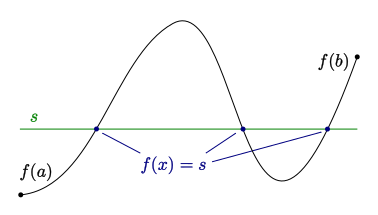
\includegraphics[scale=0.8]{Illustration_for_the_intermediate_value_theorem.png}
% \caption{intermediate value from wiki}
% \end{figure}

Dalam penggunaannya, kita cari interval sehingga salah satu ujungnya
hasil fungsinya positif dan ujung lainnya hasil fungsinya negatif,
\(u=0\) adalah nilai yang dicari. Eksistensi nilai \(u\) dijamin oleh
teorema nilai antara sebab \(a\) dan \(b\) berbeda tanda. Kemudian yang
dilakukan adalah mencari titik tengah antara \(a\) dan \(b\), sebut saja
\(c\), lalu melihat tanda dari \(f(c)\) apakah sama dengan tanda
(\emph{sign}) \(f(a)\) atau tanda \(f(b)\). Jika sama dengan tanda
\(f(a)\), maka \([c,b]\) adalah interval baru yang dicari, kalau tidak,
maka \([a,c]\) adalah interval baru yang dipilih. Proses ini diulangi
sampai kita mendapatkan toleransi yang diinginkan.

\begin{figure}
\centering
\includegraphics[scale=0.5]{412px-Bisection_method.svg.png}
\caption{Biseksi}
\end{figure}

    \hypertarget{algoritma}{%
\subsection{Algoritma}\label{algoritma}}

    Metode biseksi bisa ditulis dengan \emph{pseudocode} sebagai berikut.

    \begin{verbatim}
INPUT: Fungsi f, ujung interval LOW, HIGH, toleransi TOL, iterasi maksimum MAX
SYARAT AWAL: a < b,  f(a) * f(b) < 0 
OUTPUT: nilai yang selisihnya dengan akar f(x)=0 kurang dari TOL
 
N ← 1
While N ≤ NMAX 
  MID ← (LOW+HIGH)/2 
  If f(MID) = 0 or (HIGH-LOW)/2 < TOL then # MID adalah solusi
    Output(MID)
    Stop
  EndIf
  N ← N + 1 # increment step counter
  If (f(MID)*(f(LOW)>0 then LOW ← MID else HIGH ← MID # interval baru
EndWhile
Output("Metode biseksi gagal.") # Maksimum iterasi tercapai
\end{verbatim}

    \hypertarget{error-dan-konvergensi}{%
\subsection{Error dan Konvergensi}\label{error-dan-konvergensi}}

    Pada metode biseksi, eksistensi akar dijamin ada oleh teorema nilai
antara, hanya bila fungsi yang dicari akarnya kontinu serta kedua ujung
interval nilai fungsinya berbeda tanda. Jadi dengan memilih interval
awal yang tepat, kita selalu bisa mendekati akar yang diinginkan. Namun
demikian, laju kekonvergenan fungsi ini hanyalah linear sebab pada
setiap iterasi, kemungkinan eror hanya berkurang setengahnya. Misalkan
\(f\) adalah fungsi yang dicari akarnya, \(c\) adalah akar dari \(f\),
dan \(c_n\) adalah tebakan ke \(n\) dari metode biseksi (yaitu MID),
maka berlaku \$ \textbar c\_n -c\textbar{} \textless{}
\textbar a-b\textbar/2\^{}n\$. Nilai absolut eror selalu berkurang
setengah untuk setiap iterasi. Akibatnya metode biseksi ini konvergen
secara linear dengan faktor \(1/2\). Persamaan tersebut juga bisa
digunakan untuk menentukan kira-kira berapa banyak iterasi yang
dibutuhkan untuk konvergen ke solusi.

Misalkan \(\varepsilon\) adalah eror yang diperbolehkan dan \(n\) adalah
banyak iterasi. Berlaku


\begin{align}
|c_n - c| < |a-b|/2^n &\iff 2^n < \frac{|a-b|}{|c_n - c|} \\ 
&\iff n < \log_2 \left(\frac{\varepsilon_0}{ \varepsilon} \right) = \frac{\log \varepsilon_0 - \log \varepsilon}{\log 2}
\end{align}

    \hypertarget{latihan}{%
\subsection{Latihan}\label{latihan}}

    \begin{enumerate}
\def\labelenumi{\arabic{enumi}.}
\tightlist
\item
  Buatlah fungsi biseksi dengan input interval ({[}LOW,HIGH{]}), fungsi
  (F), dan toleransi (TOL).
\item
  Tentukan salah satu akar dari persamaan \(x^3 - x -2 =0\) serta rekam
  semua tebakan (LOW,MID,HIGH) dalam satu tabel. Perlihatkan pula bahwa
  nilai iterasi yang didapat tidak melebihi estimasi banyak iterasi pada
  persamaan (*)
\item
\end{enumerate}


    % Add a bibliography block to the postdoc
    
    
    
